\documentclass[12pt]{article}
\usepackage{amsfonts}
\usepackage{fancyhdr}
\usepackage{comment}
\usepackage[a4paper, top=2.5cm, bottom=2.5cm, left=2.2cm, right=2.2cm]%
{geometry}
\usepackage{times}
\usepackage{amsmath}
\usepackage{changepage}
\usepackage{amssymb}
\usepackage{fixltx2e}
\usepackage{enumerate}
\usepackage{graphicx}
\usepackage{float}
\newtheorem{theorem}{Theorem}
\newtheorem{acknowledgement}[theorem]{Acknowledgement}
\newtheorem{algorithm}[theorem]{Algorithm}
\newtheorem{axiom}{Axiom}
\newtheorem{case}[theorem]{Case}
\newtheorem{claim}[theorem]{Claim}
\newtheorem{conclusion}[theorem]{Conclusion}
\newtheorem{condition}[theorem]{Condition}
\newtheorem{conjecture}[theorem]{Conjecture}
\newtheorem{corollary}[theorem]{Corollary}
\newtheorem{criterion}[theorem]{Criterion}
\newtheorem{definition}[theorem]{Definition}
\newtheorem{example}[theorem]{Example}
\newtheorem{exercise}[theorem]{Exercise}
\newtheorem{lemma}[theorem]{Lemma}
\newtheorem{notation}[theorem]{Notation}
\newtheorem{problem}[theorem]{Problem}
\newtheorem{proposition}[theorem]{Proposition}
\newtheorem{remark}[theorem]{Remark}
\newtheorem{solution}[theorem]{Solution}
\newtheorem{summary}[theorem]{Summary}
\newenvironment{proof}[1][Proof]{\textbf{#1.} }{\ \rule{0.5em}{0.5em}}

\newcommand{\Q}{\mathbb{Q}}
\newcommand{\R}{\mathbb{R}}
\newcommand{\C}{\mathbb{C}}
\newcommand{\Z}{\mathbb{Z}}

\begin{document}

\title{SIE 545: Fundamentals of Optimization \\Homework 1}
\author{Martin Manuel Lopez \\lopez9@email.arizona.edu \\Systems and Industrial Engineering}
\date{\today}
\maketitle
\section{Problem 1}   
(Facility location problem) Suppose we are given n potential facility
locations and a list of m clients who need to be serviced from these lo-
cations. There is a xed cost cj of opening a facility at location j, while
there is a cost of dij of serving client i from facility j. The goal is to se-
lect a set of facility locations and assign each client to one facility, while
minimizing the total cost. Formulate this problem into an optimization
problem by the 4 steps introduced in class.

\subsection{Problem Data}
    \begin{equation*}
        \begin{split}
            &n  = \text{potential facility locations}\\
            &m  = \text{number of clients that need to be served}\\
            &C_j  = \text{Opening cost for a facility}\\
            &d\textsubscript{ij} = \text{Cost of serving client \textit{i} in facility \textit{j}}\\  
        \end{split}
    \end{equation*}
\subsection{Decision Variables}
    \begin{align*}
        &y_j \in 
            \begin{cases} 
                1 & \text{Opening facility at location} j\\
                0 & \text{otherwise}\\
            \end{cases}
        \\ %paragraph break
        \\
        &x\textsubscript{ij} \in
            \begin{cases}
                1 & \text{Assigning client } i \text{to location } j\\
                0 & \text{otherwise}\\
            \end{cases}
    \end{align*}

\subsection{Objective Function}
    \begin{equation*}
       \min \sum_{j=1}^{n} y_jC_j + \sum_{i=1}^{m} \sum_{j=1}^{n} x\textsubscript{ij}d\textsubscript{ij}
    \end{equation*}

\subsection{Constraints}
    \begin{align*}
        &\text{Client must be serviced:}\\
        &\sum_{j=1}^{n} x\textsubscript{ij} = 1 \quad \forall i,...,m\\ \\
        &\text{Clients cannot be serviced if location is not open:}\\
        &x\textsubscript{ij} \leq y_i\\ \\
        &x\textsubscript{ij} \in \text{{0,1}}\\
        &y_j \in \text{{0,1}} \forall i,j\\
    \end{align*}

\section{Problem 2}
Consider the following nonlinear programming problem:
\begin{align}
\min \quad &3x_1 + 2x_2  \\
&-x_1 + x_2^2 -4 = 0   \\
&x_1 - 1 \leq 0  \\
&x_2 \geq 0
\end{align}

Sketch the feasible region and the contours of the objective function.
Identify the optimum graphically on your sketch. Also write down the
optimal solution and the optimal objective value.

\subsection {Feasible Region}
    \begin{figure}[H]
        \centering
        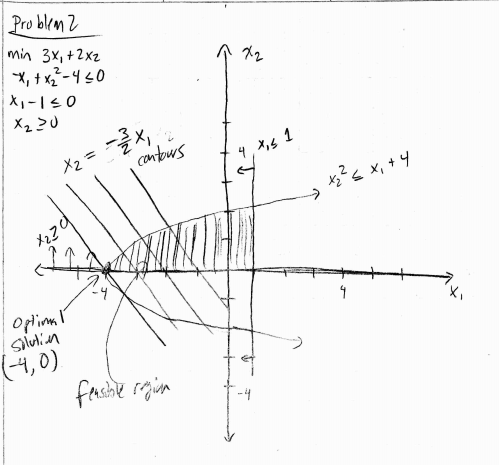
\includegraphics[width=\textwidth]{Feasible_Region.png}
        \caption{Feasible Region}
    \end{figure}

\subsection{Optimal Solution}
    \begin{align*}
        &Optimal Solution (x_1 , x_2) = (-4,0)
    \end{align*}

\subparagraph{Optimal Value:}
    \begin{align*}
        &Optimal Value: \min 3x_1 + 2x_2\\
        &\Longleftrightarrow 3(-4)+2(0) = -12\\
    \end{align*}


\section{Problem 3: BSS 1.4}
Suppose that the demand \textit{d\textsubscript{1},...,d\textsubscript{n}} for a certain product over over \textit{n} periods is known. The demand during period \textit{j} can be met from the production \textit{x\textsubscript{j}} during the period or from the warehouse stock. Any excess production can be stored at the warehouse. However, the warehouse has the capacity \textit{K}, and it would cost \textdollar c to carry over one unit from one period to another. The cost of production during period \textit{j} is given by \textit{f(x\textsubscript{j})} for \textit{j = 1,...,n}. If the initial inventory is \textit{I\textsubscript{0}},formulate the production scheduling problem as a nonlinear program. 
\subsection{Problem Data}

\subsection{Decision Variables}
\begin{equation*}
        \begin{split}
            &d_j  = \text{Demand for period } j \quad j = 1,...,n\\
            &I_j  = \text{Inventory at the end of period } j \quad j= 0,...,n\\
            &x_j  = \text{Production of units in period } j \quad j = 1,...,n\\
            &f(x_j) = \text{Cost of production of during period } j\\
            &K = \text{Warehouse capacity}\\
            &c= \text{Cost to carry over one unit from one period to the next}\\
        \end{split}
    \end{equation*}
\subsection{Objective Function}
    \begin{equation*}
       \min \sum_{j=1}^{n} [f(x_j) + cI_j]\\
    \end{equation*}
\subsection{Constraints}
    \begin{align*}
       &I_j \leq K \quad \text{for } j=1,...,n-1 \quad \text{Cannot exceed capacity of warehouse}\\
       &I_n = 0 \quad \quad \quad \quad \quad \quad \quad \quad \quad \quad \text{Demand is met by final period no inventory left}\\
       &x_j - d_j + I\textsubscript{j-1} = I_j \quad \text{for } j = 1,..,n \quad \text{Leftover inventory is after meeting demand}\\
       &x_j \geq 0 \quad \text{for } j=1,...,n-1\\
       &I_j \geq 0 \quad \text{for } J=1,..,n-1\\
    \end{align*}
    
\subsection{Nonlinear Program for 1.4}
    \begin{equation*}
       \min \sum_{j=1}^{n} [f(x_j) + cI_j]\\
    \end{equation*}
       \begin{align*} 
            &\text{Subject to}\\
            &I_j \leq K \quad \text{for } j=1,...,n-1\\
            &I_n = 0\\
            &x_j - d_j + I\textsubscript{j-1} = I_j \quad \text{for } j = 1,..,n\\
            &x_j \geq 0 \quad \text{for } j=1,...,n-1\\
            &I_j \geq 0 \quad \text{for } J=1,..,n-1\\
        \end{align*}
        
\section{Problem 4: BSS 1.7}
A household with budget \textit{b} purchases \textit{n} commodities. The unit price of commodity \textit{j} is \textit{c\textsubscript{j}}, and the minimal amount of the commodity to be purchased is $\ell$\textsubscript{j}. After the minimal amounts of the \textit{n} products are consumed, a fraction \textit{a\textsubscript{j}} of the remaining budget is allocated to commodity \textit{j}. The behavior of the household is observed over \textit{m} months for the purpose of estimating $\ell$\textsubscript{1},..., $\ell$\textsubscript{n}, and \textit{a\textsubscript{1}},...,\textit{a\textsubscript{n}}. Develop a regression model for estimating these parameters if:
\begin{enumerate}[(a)]
\item The sum of the squares of the error is to be minimized.
\item The maximum absolute value of the error is to be minimized
\item The sum of the absolute values of the error is to be minimized
\item For both parts b an c, reformulate the problems as linear programs.
\end{enumerate}

\subsection{BSS 1.7 (A): Sum of squares of the error is minimized}
\subsubsection{Problem Data}

\subsubsection{Decision Variables}

\subsubsection{Objective Function}

\subsubsection{Constraints}

\subsection{BSS 1.7 (B): Max absolute value of error is minimized}
\subsubsection{Problem Data}

\subsubsection{Decision Variables}

\subsubsection{Objective Function}

\subsubsection{Constraints}

\subsection{BSS 1.7 (C): Sum of absolute values of errors minimized}
\subsubsection{Problem Data}

\subsubsection{Decision Variables}

\subsubsection{Objective Function}

\subsubsection{Constraints}

\subsection{BSS 1.7 (D): Reformulations of b and c}
\subsubsection{Problem Data}

\subsubsection{Decision Variables}

\subsubsection{Objective Function}

\subsubsection{Constraints}


\subsection{Reformulations}
Given  \( f_i \in \realnumbers, x_i \in \realnumbers and w_i \in \realnumbers \) for \( i = 1,...m \) formulate the following minimization problem:\\
\begin{equation*}
    \min_{a_0,a_1,...,a_n} \sum_{i=1}^{m} w_i \mid f_i -  (a_0 + a_1 x_i + ... + a_nx_i^n \mid
\end{equation*}
as a (mixed integer) \textit{linear programming} problem. (Hint: the coefficients \( w_i (i = 1,...,m) \) could be positive or negative).

\subsubsection{Solution}
\end{document}